\chapter{光线追踪}

\section{Shadow Mapping}

经典的shadow mapping只能处理点光源

点光源下如何生成阴影?

\begin{enumerate}
    \item Render from light 从光源看向场景记录看到的深度。
    \item Projec to light 投影回光源
\end{enumerate}

阴影图的问题,只能做\textsl{硬阴影},做不了\textsl{软阴影},物理上区分阴影:\textsl{本影}和\textsl{半影}

\section{为什么需要光线追踪}

光栅化着色只考虑光线至弹射一次,难以解决光线弹射很多次的情况。

光栅化快但是质量低

\section{光线}

基本假设:光线沿直线传播,光路可逆

\section{Ray Casting}

从摄影机连一条线穿过像素到达物体上的点,在连接光源和点,由于光路可逆性,这就是光源到眼睛的的光的路径。

\subsection*{Pinhole Camera Model}

\section{Recursive(Whitted-Style) Ray Tracing}

弹射后的能量损失

\section{光线与物体表面交点怎么求?}

\subsection*{Ray Equation}

\begin{equation}
    \mathbf{r}(t)=\mathbf{o}+t\mathbf{d}\ \ \ \ 0\leqslant t\leqslant \infty
\end{equation}

\subsection*{Ray Intersection With Sphere}

\subsection*{Ray Intersection With Implicit Sufaces}

\subsection*{Ray Intersection With Triangle Mesh}

在图形内发射一条光线,和图形边界的交点一定是奇数,在图形外交点一定是偶数。

由于三角形一定在一个平面内,首先求光线和平面求交,然后在判断这个点是否在三角形内部。

\textsl{平面方程}形式如下
\begin{equation}
    \mathbf{p}:(\mathbf{p}-\mathbf{p}')\cdot \mathbf{N}=0
\end{equation}

其中$\mathbf{N}$为平面的法线。

下面求与平面的交点

完成了上面一步,下面就是怎么判断这个点在三角形内部,怎么判断这个点在三角形内部呢?\textsl{M$\ddot{o}$ller Trumbore Algorithm},用重心坐标
\begin{equation}
    \overrightarrow{\mathbf{O}}+t\overrightarrow{\mathbf{D}}=(1-b_1-b_2)\overrightarrow{\mathbf{P}}_0
    +b_1\overrightarrow{\mathbf{P}}_1+b_2\overrightarrow{\mathbf{P}}_2
\end{equation}

写成矩阵形式

\section{Accelerating Ray-Sufaces Intersection}

怎么样去加速?

\subsection*{Bounding Volumes}

思路是如果一个光线连包围盒都碰不到,那根本不可能碰到里边的物体

\textsl{轴对齐包围盒(Axis-Aligned Bounding Box AABB)}

如何判定光线和盒子有没有交点呢?

只有当光线进入盒所有的三个对面,那就是进入了盒子,只要离开了任意一个对面,那就算离开。

光线和AABB有交点当且仅当
\begin{equation}
    t_{enter}<t_{exit}\ \ \  and\ \ \ t_{exit}>=0
\end{equation}

\section{Uniform Spatial Partitions(Grids)}

\subsection*{Ray-Scene Intersection}

只需要做若干次光线和盒子求交

格子的数量不能太稀疏,也不能太密集

“Teapot in a stadium ” problem

\section{Spatial Partitions}

在稀疏的地方不需要这么多个格子。
\begin{figure}[H]
    \centering
    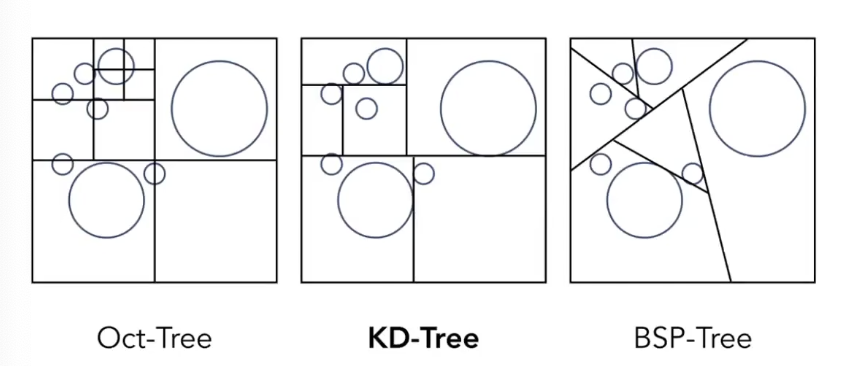
\includegraphics[scale=0.4]{figures/空间划分.png}
    \caption{空间划分方法}
\end{figure}

\subsection*{KD-Tree}

kd-tree是在光线追踪之前做好。

每次找到格子,总是沿着某一个轴砍一刀,就砍一刀。

\subsection*{KD-tree Pre-Processing}

\begin{figure}[H]
    \centering
    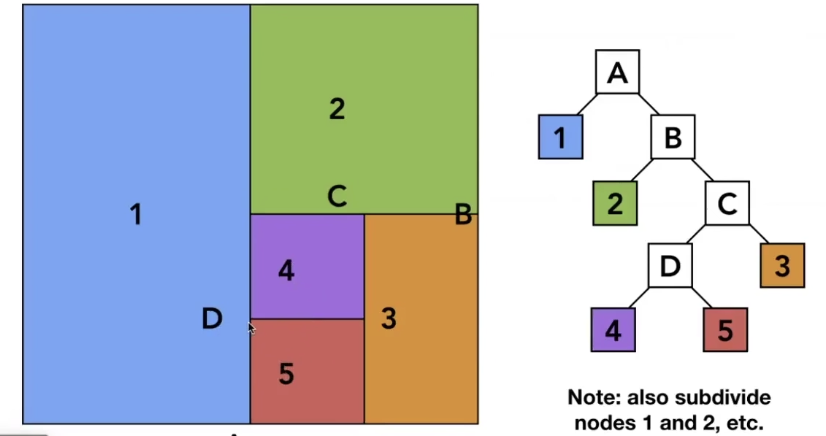
\includegraphics[scale=0.4]{figures/KD-tree.png}
    \caption{KD-tree}
\end{figure}

对于任意一个节点,沿着哪个轴划分,然后划分在哪儿。

\subsection*{Travering a KD-Tree}

\subsection*{KD-Tree的问题}

怎么判定三角形的交集

\section{Object Partition and Bounding Volume Hierarchy}

\subsection*{Bounding Volume Hierarchy(BVH)}

解决KD-Tree三角形的问题。完全省去三角形与包围盒求交点

把三角形分为两部分,重新设置包围盒。

\begin{figure}[H]
\centering
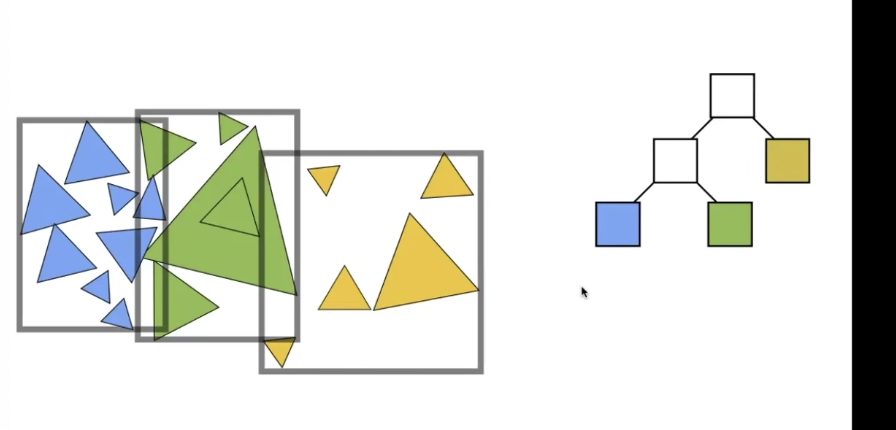
\includegraphics[scale=0.4]{figures/BVH.png}
\caption{BVH}
\end{figure}

BVH的性质:一个物体只在一个盒子里

BVH对空间的划分不是完全划分开,Box可以相交。

\subsection*{Summary:building BVH}

技巧:快速划分算法,受到快速划分启发。

技巧2:永远沿着最长的轴,中位数

\subsection*{BVH Traversal}




